\subsection*{Model}
The function described in this problem is the following
\begin{equation*}
    \begin{aligned}
    & F(\mathbf{x}) = \frac{1}{2} \sum_{k=1}^{n} f_k^2(x) \\
    & f_k(\mathbf{x}) = x_k - \frac{x_{k+1}^2}{10}, \quad   1 \leq k < n \\   
    & f_n(\mathbf{x}) = x_n - \frac{x_1^2}{10}
    \end{aligned}
\end{equation*}
where $n$ denotes the dimensionality of the input vector $\mathbf{x}$.
\\ The starting point for the minimization is the vector $\mathbf{x}_0 = [2, 2, \ldots, 2]$.


To be able to say something more about the behaviour of the problem is useful to look at the gradient of the function $F(\mathbf{x})$ and at its Hessian matrix.
\begin{equation*}
    \nabla F(\mathbf{x}) = 
    \begin{bmatrix}
        \frac{\partial F}{\partial x_1}(\mathbf{x}) \\
        \vdots \\
        \frac{\partial F}{\partial x_k}(\mathbf{x}) \\
        \vdots \\
        \frac{\partial F}{\partial x_n}(\mathbf{x})
    \end{bmatrix}
    =
    \begin{bmatrix}
        \frac{\partial}{\partial x_1} \frac{1}{2}\left[f_n^2 + f_1^2\right] (\mathbf{x})\\
        \vdots \\
        \frac{\partial}{\partial x_k} \frac{1}{2}\left[f_{k-1}^2 + f_k^2\right] (\mathbf{x})\\
        \vdots \\
        \frac{\partial}{\partial x_n}  \frac{1}{2}\left[f_{n-1}^2 + f_n^2\right] (\mathbf{x})
    \end{bmatrix}
    =
    \begin{bmatrix}
        -\frac{x_1}{5}\left(x_n - \frac{x_1^2}{10}\right) + \left(x_1 - \frac{x_1^2}{10}\right) \\
        \vdots \\
        -\frac{x_k}{5}\left(x_{k-1} - \frac{x_k^2}{10}\right) + \left(x_k - \frac{x_{k+1}^2}{10}\right) \\
        \vdots \\
        -\frac{x_n}{5}\left(x_{n-1} - \frac{x_n^2}{10}\right) + \left(x_n - \frac{x_1^2}{10}\right)
    \end{bmatrix}
\end{equation*}
Due to the particular structure of the function, the Hessian matrix as a sparse structure, with only 3 diagonals different from zero. The non-zero elements are the following:
\begin{align*}
    \frac{\partial^2 F}{\partial x_k^2} (\mathbf{x}) &= -\frac{1}{5}x_{k-1} - \frac{3}{50}x_k^2  + 1, \quad 1 < k \leq n  &
    \frac{\partial^2 F}{\partial x_1^2} (\mathbf{x}) &= -\frac{1}{5}x_{n} - \frac{3}{50}x_1^2  + 1, \\
    \frac{\partial^2 F}{\partial x_k \partial x_{k+1}} (\mathbf{x}) &= -\frac{1}{5}x_{k+1}, \quad 1 \leq k < n  &
    \frac{\partial^2 F}{\partial x_n \partial x_1}(\mathbf{x}) &= -\frac{1}{5}x_1  \\
    \frac{\partial^2 F}{\partial x_k \partial x_{k-1}}(\mathbf{x}) &= -\frac{1}{5}x_{k}, \quad 1 < k \leq n  &
    \frac{\partial^2 F}{\partial x_1 \partial x_{n}}(\mathbf{x}) &= -\frac{1}{5}x_{n}
\end{align*}
We can now easily notice that the gradient of the function is null when all the components of the vector $\mathbf{x}$ are equal to 0. The Hessian matrix is positive definite, so the point $\mathbf{x} = \mathbf{0}$ is a minimum of the function $F(\mathbf{x})$. 
Because of the definition of the function, $0$ is the lowest value that the function can assume, so the minimum is global.


\subsection*{Nealder Mead Method}
We now report a table containing some general results obtained by running the Nealder Mead method on the function $F(\mathbf{x})$.

\begin{figure*}[htbp]
    \centering
    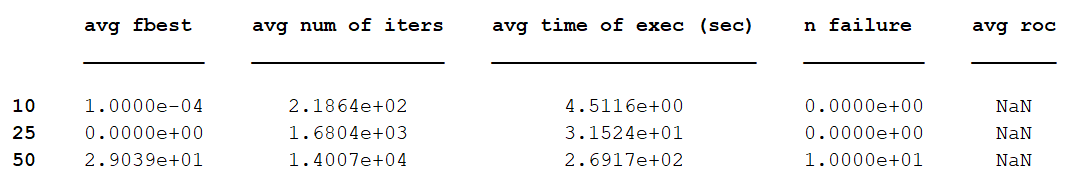
\includegraphics[width = 0.9\textwidth]{img/pb76_table_SX.png}
    \caption{Resultats obtained by running the symplex method on the function $F(\mathbf{x})$.}
\end{figure*}

First thing we can notice is that for smaller dimensionalities the symplex method is able to find the minimum in a reasonable amount of time, but when the dimensionality becomes higher the method starts failing.
From the plot in figure $\eqref{fig:iter}$, we can see that for most points belonging to $\mathbb{R}^{50}$, the method keeps iterating until the maximum number of iterations is reached without satisfying the stopping criterion.
This behaviour can probably be explained by the fact that when the dimensionality increases the starting point is more far from the minimum due to its definiotion, so the method needs to perform more iterations to reach the minimum.
\begin{figure}[htbp]
    \centering
    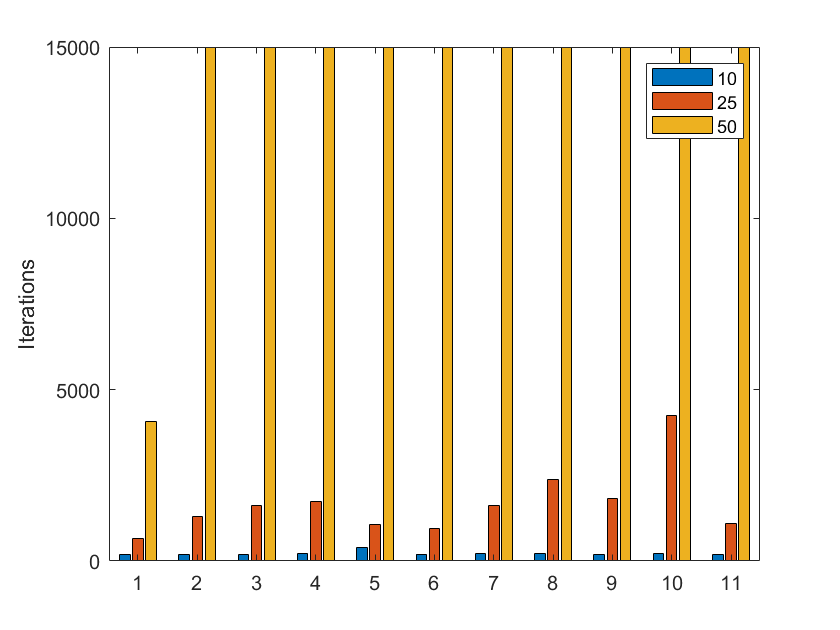
\includegraphics[width = 0.5\textwidth]{img/pb76_SX_iter.png}
    \caption{Number of iterations needed by the Nealder Mead method to find the minimum of the function $F(\mathbf{x})$ for each starting point.}
    \label{fig:iter}
\end{figure}


\subsection*{Modified Newton Method}
We now report a table containing some general results obtained by running the Modified Newton method on the function $F(\mathbf{x})$.
We obviously expect the method to perform better than the symplex method because of the exact derivatives used in the computation of the descent direction.

\begin{figure*}[htbp]
    \centering
    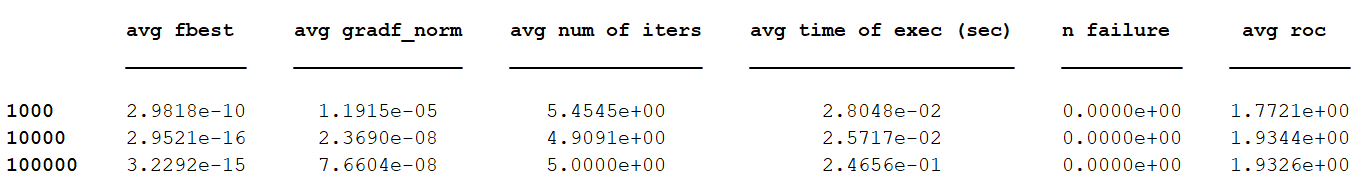
\includegraphics[width = 0.9\textwidth]{img/pb76_table_MN.png}
    \caption{Resultats obtained by running the Modified Newton Method on the function $F(\mathbf{x})$ using the exact derivatives.}
\end{figure*}

This time, the method always converges to the minimum in very few iterations, even for higher dimensionalities. 